\documentclass[border=10pt]{standalone}
\usepackage{amsmath,amssymb}
\usepackage{xcolor}
\usepackage{tikz}
\usetikzlibrary{shapes,arrows.meta,positioning,fit,backgrounds,calc,decorations.pathreplacing}

% Color palette
\definecolor{cmpcolor}{HTML}{7B68EE}    % Medium slate blue for CMP
\definecolor{rrdcolor}{HTML}{9370DB}     % Medium purple for RRD
\definecolor{condcolor}{HTML}{3CB371}    % Medium sea green for condition encoder
\definecolor{tokencolor}{HTML}{FF8C00}   % Dark orange for tokens
\definecolor{losscolor}{HTML}{DC143C}    % Crimson for loss
\definecolor{sscolor}{HTML}{4682B4}      % Steel blue for scheduled sampling
\definecolor{bgstage}{HTML}{F5F0FF}      % Light purple background

\begin{document}
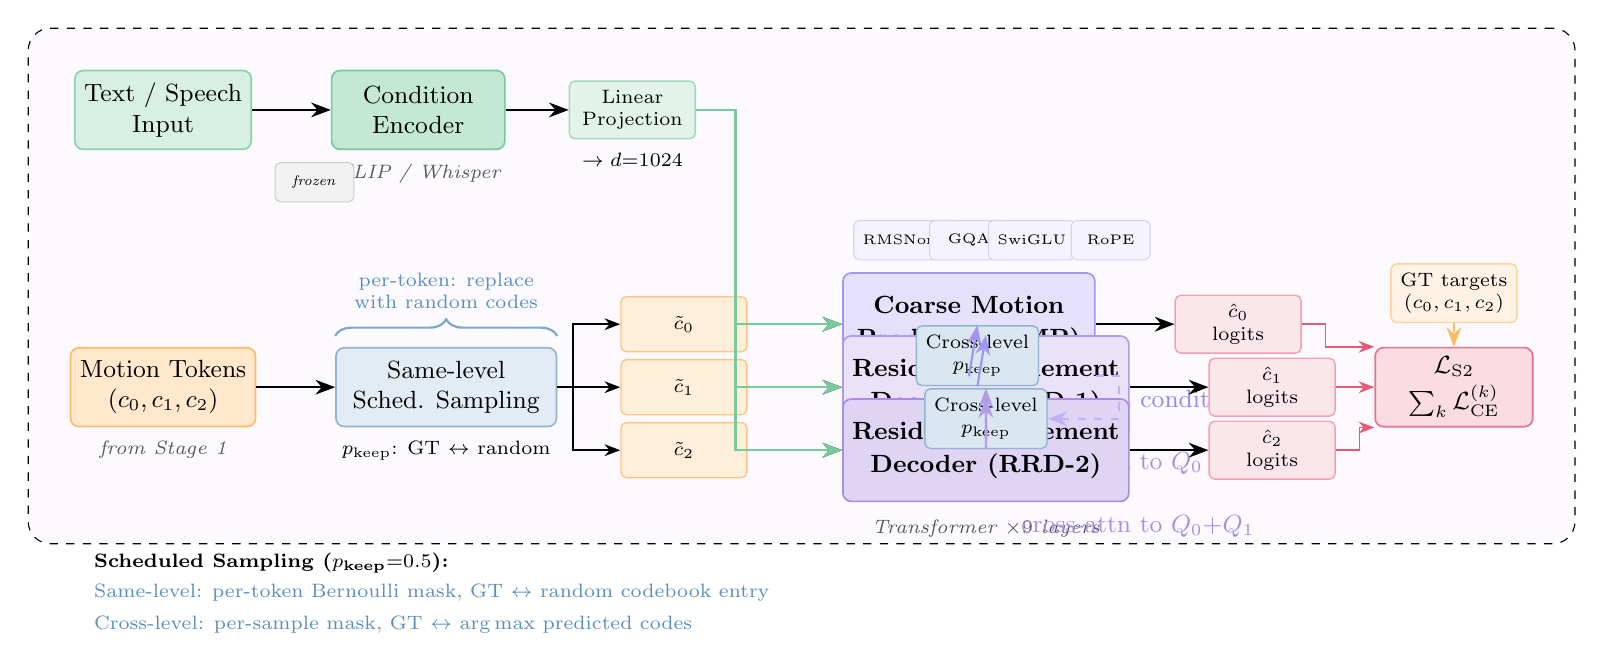
\begin{tikzpicture}[
    node distance=0.7cm and 1.0cm,
    block/.style={rectangle, draw, rounded corners=3pt, minimum height=1.0cm, minimum width=2.2cm, align=center, font=\small, line width=0.6pt},
    smallblock/.style={rectangle, draw, rounded corners=2pt, minimum height=0.7cm, minimum width=1.6cm, align=center, font=\scriptsize, line width=0.5pt},
    tinyblock/.style={rectangle, draw, rounded corners=2pt, minimum height=0.5cm, minimum width=1.0cm, align=center, font=\tiny, line width=0.4pt},
    arrow/.style={-{Stealth[length=2.5mm]}, thick},
    dasharrow/.style={-{Stealth[length=2.5mm]}, thick, dashed},
    thinarrow/.style={-{Stealth[length=2mm]}, semithick},
    label/.style={font=\scriptsize\itshape, text=gray!70!black},
    mathlabel/.style={font=\scriptsize, text=black},
]

% ============================================================
%  INPUT SECTION
% ============================================================

% Condition input
\node[block, fill=condcolor!20, draw=condcolor!60] (cond_input) {Text / Speech\\Input};

% Condition encoder
\node[block, fill=condcolor!30, draw=condcolor!70, right=1.0cm of cond_input] (cond_enc) {Condition\\Encoder};
\node[label, below=0.05cm of cond_enc] {CLIP / Whisper};
\node[tinyblock, fill=gray!10, draw=gray!40, below left=0.15cm and -0.3cm of cond_enc] (frozen1) {\textit{frozen}};

\draw[arrow] (cond_input) -- (cond_enc);

% Projection
\node[smallblock, fill=condcolor!15, draw=condcolor!50, right=0.8cm of cond_enc] (proj) {Linear\\Projection};
\node[mathlabel, below=0.05cm of proj] {$\rightarrow d{=}1024$};

\draw[arrow] (cond_enc) -- (proj);

% Motion tokens input
\node[block, fill=tokencolor!20, draw=tokencolor!60, below=2.5cm of cond_input] (tokens_in) {Motion Tokens\\$(c_0, c_1, c_2)$};
\node[label, below=0.05cm of tokens_in] {from Stage 1};

% ============================================================
%  SAME-LEVEL SCHEDULED SAMPLING
% ============================================================

\node[block, fill=sscolor!15, draw=sscolor!60, right=1.0cm of tokens_in, minimum width=2.8cm] (same_ss) {Same-level\\Sched. Sampling};
\node[mathlabel, below=0.05cm of same_ss] {$p_\text{keep}$: GT $\leftrightarrow$ random};

\draw[arrow] (tokens_in) -- (same_ss);

% Split tokens
\node[smallblock, fill=tokencolor!15, draw=tokencolor!50, right=0.8cm of same_ss, yshift=0.8cm] (tok_q0) {$\tilde{c}_0$};
\node[smallblock, fill=tokencolor!15, draw=tokencolor!50, right=0.8cm of same_ss] (tok_q1) {$\tilde{c}_1$};
\node[smallblock, fill=tokencolor!15, draw=tokencolor!50, right=0.8cm of same_ss, yshift=-0.8cm] (tok_q2) {$\tilde{c}_2$};

\draw[thinarrow] (same_ss.east) -- ++(0.2,0) |- (tok_q0.west);
\draw[thinarrow] (same_ss.east) -- (tok_q1.west);
\draw[thinarrow] (same_ss.east) -- ++(0.2,0) |- (tok_q2.west);

% ============================================================
%  DECODER SECTION
% ============================================================

% Q0 Decoder - CMP
\node[block, fill=cmpcolor!20, draw=cmpcolor!70, right=1.2cm of tok_q0, minimum width=3.2cm, minimum height=1.3cm] (q0dec) {\textbf{Coarse Motion}\\[1pt]\textbf{Predictor (CMP)}};

% Architecture details for Q0
\node[tinyblock, fill=cmpcolor!8, draw=cmpcolor!30, above=0.15cm of q0dec, xshift=-0.8cm] (q0_rms) {RMSNorm};
\node[tinyblock, fill=cmpcolor!8, draw=cmpcolor!30, above=0.15cm of q0dec] (q0_gqa) {GQA};
\node[tinyblock, fill=cmpcolor!8, draw=cmpcolor!30, above=0.15cm of q0dec, xshift=0.8cm] (q0_swi) {SwiGLU};
\node[tinyblock, fill=cmpcolor!8, draw=cmpcolor!30, above=0.15cm of q0dec, xshift=1.8cm] (q0_rope) {RoPE};
\node[label, below=0.1cm of q0dec] {LlamaGen $\times 9$ layers};
\node[mathlabel, below right=0.05cm and -1.5cm of q0dec, text=cmpcolor!80] {\small prefix-concat conditioning};

% Q1 Decoder - RRD
\node[block, fill=rrdcolor!20, draw=rrdcolor!70, right=1.2cm of tok_q1, minimum width=3.2cm, minimum height=1.3cm] (q1dec) {\textbf{Residual Refinement}\\[1pt]\textbf{Decoder (RRD-1)}};
\node[label, below=0.1cm of q1dec] {Transformer $\times 9$ layers};
\node[mathlabel, below right=0.05cm and -1.5cm of q1dec, text=rrdcolor!80] {\small cross-attn to $Q_0$};

% Q2 Decoder - RRD
\node[block, fill=rrdcolor!30, draw=rrdcolor!80, right=1.2cm of tok_q2, minimum width=3.2cm, minimum height=1.3cm] (q2dec) {\textbf{Residual Refinement}\\[1pt]\textbf{Decoder (RRD-2)}};
\node[label, below=0.1cm of q2dec] {Transformer $\times 9$ layers};
\node[mathlabel, below right=0.05cm and -1.5cm of q2dec, text=rrdcolor!80] {\small cross-attn to $Q_0{+}Q_1$};

% Connect tokens to decoders
\draw[arrow] (tok_q0) -- (q0dec);
\draw[arrow] (tok_q1) -- (q1dec);
\draw[arrow] (tok_q2) -- (q2dec);

% Connect condition to all decoders
\draw[arrow, color=condcolor!70] (proj.east) -- ++(0.5, 0) |- (q0dec.west);
\draw[arrow, color=condcolor!70] (proj.east) -- ++(0.5, 0) |- (q1dec.west);
\draw[arrow, color=condcolor!70] (proj.east) -- ++(0.5, 0) |- (q2dec.west);

% ============================================================
%  CROSS-LEVEL SCHEDULED SAMPLING (between decoders)
% ============================================================

% Cross-level SS between Q0 → Q1
\node[smallblock, fill=sscolor!20, draw=sscolor!60, minimum width=1.4cm] at ($(q0dec.south)!0.5!(q1dec.north)$) (cross_ss1) {Cross-level\\$p_\text{keep}$};

\draw[arrow, color=cmpcolor!70] (q0dec.south) -- (cross_ss1.north);
\draw[arrow, color=cmpcolor!70] (cross_ss1.south) -- (q1dec.north);

% Cross-level SS between Q1 → Q2
\node[smallblock, fill=sscolor!20, draw=sscolor!60, minimum width=1.4cm] at ($(q1dec.south)!0.5!(q2dec.north)$) (cross_ss2) {Cross-level\\$p_\text{keep}$};

\draw[arrow, color=rrdcolor!70] (q1dec.south) -- (cross_ss2.north);
\draw[arrow, color=rrdcolor!70] (cross_ss2.south) -- (q2dec.north);

% Q0 also feeds Q2 (skip connection through cross_ss)
\draw[arrow, color=cmpcolor!50, dashed] (q0dec.south east) -- ++(0.3, 0) |- (cross_ss2.east);

% ============================================================
%  OUTPUT SECTION
% ============================================================

% Logits
\node[smallblock, fill=losscolor!10, draw=losscolor!40, right=1.0cm of q0dec] (logit0) {$\hat{c}_0$\\logits};
\node[smallblock, fill=losscolor!10, draw=losscolor!40, right=1.0cm of q1dec] (logit1) {$\hat{c}_1$\\logits};
\node[smallblock, fill=losscolor!10, draw=losscolor!40, right=1.0cm of q2dec] (logit2) {$\hat{c}_2$\\logits};

\draw[arrow] (q0dec) -- (logit0);
\draw[arrow] (q1dec) -- (logit1);
\draw[arrow] (q2dec) -- (logit2);

% Loss
\node[block, fill=losscolor!15, draw=losscolor!60, minimum width=2.0cm] at ($(logit1.east)+(1.5,0)$) (loss) {$\mathcal{L}_\text{S2}$\\[2pt]$\sum_{k} \mathcal{L}_\text{CE}^{(k)}$};

\draw[thinarrow, color=losscolor!70] (logit0.east) -- ++(0.3,0) |- (loss.north west);
\draw[thinarrow, color=losscolor!70] (logit1.east) -- (loss.west);
\draw[thinarrow, color=losscolor!70] (logit2.east) -- ++(0.3,0) |- (loss.south west);

% GT targets for loss
\node[smallblock, fill=tokencolor!10, draw=tokencolor!40, above=0.3cm of loss] (gt) {GT targets\\$(c_0, c_1, c_2)$};
\draw[dasharrow, color=tokencolor!60] (gt) -- (loss);

% ============================================================
%  ANNOTATIONS
% ============================================================

% Brace for scheduled sampling explanation
\draw[decorate, decoration={brace, amplitude=6pt, raise=4pt}, thick, sscolor!70]
    (same_ss.north west) -- (same_ss.north east)
    node[midway, above=10pt, font=\scriptsize, text=sscolor!90, align=center] {per-token: replace\\with random codes};

% Legend
\node[font=\scriptsize\bfseries, anchor=north west] at (-1.0, -5.5) (legend_title) {Scheduled Sampling ($p_\text{keep}{=}0.5$):};
\node[font=\scriptsize, anchor=north west, text=sscolor!90] at (-1.0, -5.9) {Same-level: per-token Bernoulli mask, GT $\leftrightarrow$ random codebook entry};
\node[font=\scriptsize, anchor=north west, text=sscolor!90] at (-1.0, -6.3) {Cross-level: per-sample mask, GT $\leftrightarrow$ $\arg\max$ predicted codes};

% Background
\begin{scope}[on background layer]
    \node[draw, dashed, rounded corners=8pt, fill=bgstage, fill opacity=0.3, inner sep=15pt,
          fit=(cond_input)(cond_enc)(proj)(tokens_in)(same_ss)(tok_q0)(tok_q2)(q0dec)(q1dec)(q2dec)(q0_rope)(logit0)(logit2)(loss)(gt)(cross_ss1)(cross_ss2),
          label={[font=\normalsize\bfseries, text=cmpcolor!80]above:{Stage 2: Hierarchical Autoregressive Transformer}}] {};
\end{scope}

\end{tikzpicture}
\end{document}
